\chapter{Methodolgy and Implementation}
	\label{chap:implementation}
	
	\section{Tools}
	
	\subsection{Programming Languages}
	
	For the implementation of our application, three primary programming languages deemed to be best suited for development. Apple's Swift programming language \cite{swift} got considered early on, due to the author's familiarisation with the programming language. The programming language gets used for creating applications for Apple's mobile and desktop operating systems, and with 1.5 billion \cite{9to5mac} iOS devices in circulation, that was a lot of potential users. Additionally, Apple's iOS devices are prevalent within most educational settings, with Apple's iPad being one of the primary go-to devices. However, due to the language not supporting key frameworks required, or providing similar alternatives, the decision to not use this language got made. 
	
	We then got presented with three main options to use, Python, R and HTML, CSS and JavaScript.
	
	Python is a very popular programming language \cite{wired_python, sof_dev_servay20}, it is fast, easy-to-use, and easy-to-deploy programming language that gets widely used to develop scalable applications. Examples include YouTube, Instagram, Pinterest and SurveyMonkey \cite{hackr.io}. The Python Software Foundation state that Python is a high-level, object-orientated (OOP), interpreted language with dynamic semantics. Due to the language being a high-level, it has many built-in data structures. These features, along with the dynamic typing and dynamic binding together make Python attractive to development teams working in a Rapid Application Development (RAD). As Python is an extracted level above the C language \cite{sto_cpython}, Python can get used as the glue that connects existing components, as well as being able to be used as a scripting language \cite{python_desc}. Python gets considered to be easy to learn the language due to its high readability and is recommended by many exam boards as the language to use for teaching Computer Science at GCSE and A-Level level \cite{list exam boards here}. Python's simple and easy to learn syntax emphasises on readability, which, as a result, reduces the cost of program maintenance \cite{python_desc, pyqt_rbc}. 
	
	Python gets compared to a lot of other languages. However, due to the requirements and expectations of the application, we will compare it to other similar style applications that can potentially do a similar job. These being Java, JavaScript and C++. In general, the choice of the programming language to use is many other real-world constraints, for example, financial cost, availability, training and even personal preferences and attachments. However, we will focus on language issues for the comparisons.
	
	\begin{figure}[t]
		\begin{center}
			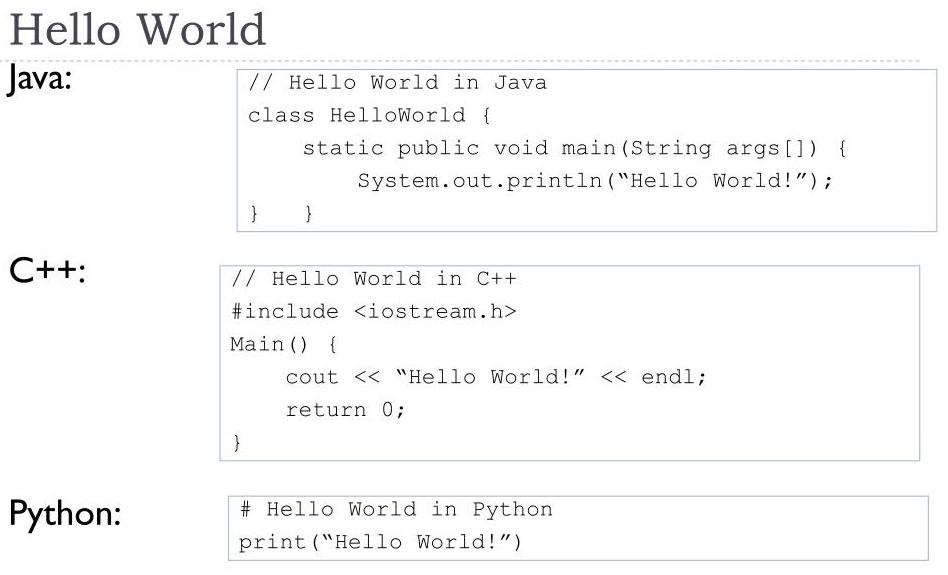
\includegraphics[width=8.5cm]{graphics/python_vs_java_vs_c++.jpg}
			\caption{A comparison between Java, Python and C++ to print an output to the console. \cite{py_ja_c++}}
			\label{fig:py_java_c++}
		\end{center}
	\end{figure}
	
	In comparison to Java, Python programs will typically take 3-5 times quicker (See fig: \ref{fig:py_java_c++}) to develop but will have a slower run time. The time difference gets attributed to Python's built-in data types and its dynamic typing \cite{python_comparison}. As Java gets better characterised as a low-level implementation language, this would be the language of choice if application execution speed was the deciding factor. If this is not a factor, then there is no real benefit over Python.
	
	What gets said about Java is also the same when comparing C++ to Python. It is often 5-10 times shorter than equivalent C++ code. Anecdotal evidence suggests that one Python programmer can finish in two months what two C++ programmers cannot complete in a year. Python shines as a glue language, used to combine components written in C++ \cite{python_comparison}.
	
	In comparison to JavaScript (JS), Python's 'object-based' subset is very similar to JS. Python supports a programming method that uses simple variables and functions, similar to JS, that do not need class definitions. However, Python also supports writing for much larger programs, which leads to more reusable code by using an accurate OOP way while with JS, that is all that it can do \cite{python_comparison}.
	
	Another language that presented itself to us was the R language. R is a language and environment for statistical computing and graphics. It is a GNU project which is similar to the S language and environment which was developed at Bell Laboratories (formerly AT\&T, now Lucent Technologies) by John Chambers and colleagues \cite{r_project}. Many users think of R as a statistics system \cite{r_project}. Academics and statisticians have developed R over two decades. There are around 12000 packages available in CRAN (open-source repository). The wide variety of library makes R the first choice for statistical analysis, especially for specialised analytical work \cite{r_vs_py}.
	
	R provides a wide variety of statistical (linear and nonlinear modelling, classical statistical tests, time-series analysis, classification, clustering) and graphical techniques, and is highly extensible. One of R's strengths is the ease with which well-designed publication-quality plots can be produced, including mathematical symbols and formulae where needed \cite{r_project}. The cutting-edge difference between R and the other statistical products is the output. R has fantastic tools to communicate the results. Rstudio comes with the library knitr. Communicating the findings with a presentation or a document is easy \cite{r_vs_py}.
	
	R and Python are both open-source programming languages with a large community. New libraries or tools are added continuously to their respective catalogue. R is mainly used for statistical analysis, while Python provides a more general approach to data science.
	R and Python are both state of the art in terms of programming language oriented towards data science. Learning both of them is, of course, the ideal solution. R and Python requires a time-investment, and such luxury is not available for everyone. Python is a general-purpose language with a readable syntax. R, however, is built by statisticians and encompasses their specific language \cite{r_vs_py}.
	
	Python can pretty much make the same tasks as R: data wrangling, engineering, feature selection web scrapping, creating an app, for example. Python is a tool to deploy and implement machine learning at a large-scale. Python codes are easier to maintain and more robust than R. Years ago; Python did not have many data analysis and machine learning libraries. 
	
	Recently, Python is catching up and provides cutting-edge API for machine learning or Artificial Intelligence. Most of the data science job can get done with five Python libraries: Numpy, Pandas, Scipy, Scikit-learn and Seaborn \cite{r_vs_py}.
	
	Python, on the other hand, makes replicability and accessibility easier than R., if we need to use the results of our analysis in an application or website, Python is the best choice \cite{r_vs_py}.
	
	In 2019 there was an active number of 26.66 billion devices attached to the internet \cite{securitytoday, statista_iot}, with an estimation of 35 billion in 2021 \cite{securitytoday} and by 2025 75.44 billion \cite{statista_iot}. Experts estimate that the IoT device market will reach \$1.1 trillion in 2026 \cite{securitytoday}. Every Second 127 new devices get connected to the world wide web \cite{securitytoday}.
	
	With so many devices on the internet, an important consideration we had was to make the application web-based. By creating the application for the internet, this would allow potentially many more people to be able to access the application and interact with the different ML models. 
	
	JS gets regarded as more of the language of the world-wide-web \cite{web_foundation}. It got initially designed to be used client-side in a web browser. However, it has in more recent years started to branch out and be able to be used to create applications on, not only the front end of the web but also desktops, servers and mobile platforms natively. For example, React Native, Node.js and TypeScript. JavaScript is also incredibly useful, allowing developers to be able to create apps with audiences in the millions quickly \cite{js_springboard}.
	
	The decision on what language to use we a close call between Python and JavaScript, this was due to the massive amounts of libraries that were on offer and the support communities that were in place. With both being open source and both having essential libraries available to interact with machine learning models and visualisation tools, both could have been a perfect fit for the intended application. However, we decided upon using Python. Python was chosen based on it being the go-to language for anything machine learning related, and its ability to be able to be used multiplatform on desktops or mobile devices. Python supports modules and packages, which encourages programs to be developed modularity and therefore allows code to get reused. The Python interpreter and the extensive standard library are available in source or binary form without charge for all major platforms and can get freely distributed \cite{python_desc}. There was also an additional factor that the author was more familiar with Python and its required libraries compared to the libraries that will get required for using JavaSript.

	There was the additional decision to use HTML and CSS within a small part of the project, the 'Learning Zone', based on the quickness of being able to create and host the webpages containing the learning content. It was allowing the learning content to evolve without having any impact on the overall development of the main application, allowing the learning content to be an individual entity within the main application.
		
		
	\section{Frameworks}
	
	\subsection{GUI Framework}
	
	With the nature of the application, we needed to make the application have a Graphical User Interface (GUI). Having a GUI allowed the learning to be a lot more hands-on and allow the players to see what is happening within the models, especially when they interact with them.
	
	Therefore, due to the GUI requirement, three GUI libraries presented themself to us. These were Pygame, PyQT5 and Tkinter.
	
	Pygame is a free, open-sourced library. Released under the LGPL licence, Pygame is a set of Python modules designed for writing video games. Pygame adds functionality on top of the standard Python library. Pygame allows the user to create fully featured games and multimedia programs in the python language \cite{pygame_wiki}.
	
	Pygame is highly portable and runs on nearly every platform and operating system, and it gets downloaded millions of times \cite{pygame_wiki}. 
	
	With the main aim of the application to be a game, Pygame was a strong contender. It was providing modules that can handle a lot of the key gaming mechanics and multiple screen switching. However, it lacked some key features that were deemed essential for the application. It was unable to provide a library that could create interactable graphs to be used as data inputs for the models and be able to render HTML and CSS content for the Learning Zone. Therefore reducing the amount of flexibility, it got decided upon for using HTML and CSS for the learning content. Therefore, meaning that all the content would need to be hardcoded. If any changes were needed, a significant transformation would need to happen to the overall code, instead of just changing the web content.
	
	PyQt is a set of Python v2 and v3 bindings for The Qt Company's Qt application framework and runs on all platforms supported by Qt including Windows, macOS, Linux, iOS and Android. PyQt5 supports Qt v5. PyQt4 supports Qt v4 and will build against Qt v5. The bindings are implemented as a set of Python modules and contain over 1,000 classes \cite{pyqt_rbc}. PyQt brings together the Qt C++ cross-platform application framework and the cross-platform interpreted language Python.
	
	Qt is more than a GUI toolkit. It includes abstractions of network sockets, threads, Unicode, regular expressions, SQL databases, SVG, OpenGL, XML, a fully functional web browser, a help system, a multimedia framework, as well as a rich collection of GUI widgets. Qt classes employ a signal/slot mechanism for communicating between objects that is type safe but loosely coupled making it easy to create re-usable software components \cite{pyqt_rbc}. Qt also includes Qt Designer, a graphical user interface designer. PyQt is able to generate Python code from Qt Designer. It is also possible to add new GUI controls written in Python to Qt Designer \cite{pyqt_rbc}. PyQt combines all the advantages of Qt and Python. A programmer has all the power of Qt but can exploit it with the simplicity of Python \cite{pyqt_rbc}.
	
	Tkinter is the third option. Tkinter commonly comes bundled with Python, using Tk and is Python's standard GUI framework. It is famous for its simplicity and graphical user interface. It is open-source and available under the Python License \cite{data_camp_gui}.
	
	Tkinter is Python's de-facto standard GUI (Graphical User Interface) package. It is a thin object-oriented layer on top of Tcl/Tk. Tkinter is not the only GuiProgramming toolkit for Python. It is however the most commonly used one. CameronLaird calls the yearly decision to keep TkInter "one of the minor traditions of the Python world \cite{py_tkinter}." Tkinter supports functionality with Matplotlib, with Matplotlib offering libraries to allow handling the backend of the graph creation interacting with the GUI library. However, unlike QT, Tkinter does not support any GUI designer. Therefore the GUIs will have to be created programmatically, which will give more control, might involve more of a learning curve and potentially more time to implement in the initial stages.
	
	After reviewing the different GUI libraries, PyQt was the decided library to use. We believed it would give us the ability to have 
	
	
	\section{Packages}
	\label{sec:packages_used}
	
	In order to create the application, there are several Python libraries required. The main one being PyQT5 \cite{pyqt_rbc}, as explained previously, to be able to create the GUI for the application. Matplotlib's \cite{hunter2007matplotlib} Backend handler for PyQT5 is another critical library required for the application. This library handled the interactions between the GUI and the interactable graphs needed for the models. TO create the models, the Sci-Kit Learn library created the Linear Regression, K-Means, GMM, SVM models while TensorFlow enables the dense Neural Network to get created \cite{tensorflow2015-whitepaper}. Two additional packages required are Numpy \cite{walt2011numpy} and Pandas, these helped manage the data and manipulate it to prepare it for the different models.
	
	\section{IDE}
	\label{sec:ide_used}
	
	PyCharm is a dedicated Python Integrated Development Environment (IDE) providing a wide range of essential tools for Python developers, tightly integrated to create a convenient environment for productive Python, web, and data science development \cite{pycharm_get_started}. While PyCharm is a very popular IDE, and one that we have had experience with before, it is not, however, one that we have had many experiences using compared to other IDEs. While it does provide much functionality and it a lot easier to use and keep our directories organised compare to Python's provide IDE, it has, however, not been an IDE that has flowed well when we have used it.
	
	Visual Studio Code (VS Code) is a free source-code editor made by Microsoft for Windows, Linux and macOS. Features include support for debugging, syntax highlighting, intelligent code completion, snippets, code refactoring, and embedded Git. Visual Studio Code combines the simplicity of a source code editor with powerful developer tooling, like IntelliSense code completion and debugging. First and foremost, it is an editor that gets out of the user's way. The delightfully frictionless edit-build-debug cycle means less time fiddling with the required environment, and more time executing ideas \cite{vs_code}.
	
	Microsoft claims that VS Code, at its heart, lightning-fast code features a lightning-fast source code editor, which is perfect for day-to-day use. With support for hundreds of languages, VS Code helps the user be instantly productive with syntax highlighting, bracket-matching, auto-indentation, box-selection, snippets, and more \cite{vs_code}. For serious coding, the user will often benefit from tools with more code understanding than just blocks of text. Visual Studio Code includes built-in support for IntelliSense code completion, rich semantic code understanding and navigation, and code refactoring \cite{vs_code}. Which we can say from experience is mostly true. However, on occasions, it has provided code completion that was not intended or needed. VS Code also allows the user to customise every feature to their liking and install any number of third-party extensions. While most scenarios work "out of the box" with no configuration, VS Code also grows with you \cite{vs_code}. Which, from our experience, we can say is true. VS Code has grown with us. The VS Code community has provided many extensions that have helped with our workflow. 
	
	Atom is developed and released by GitHub \cite{atom_explain}. Atom is free, and an open-sourced code editor. Atom is a self-labelled 'a hackable text editor for the 21st century'. Atom, like VS Code, allows developers to fully customise the look, feel, and requirements to speed up their workflows. However, Atom still allows developers to use it productively without ever touching a config file. Atom comes pre-loaded with eight syntax themes and four UI, two light and two dark, but if none of them provides any interest, Atom makes it easy and quick to install customised themes created by a third-party or to create one \cite{atom_explain}. However, apart from pre-created extensions to help with code linting and code autocomplete abilities, none of these features is of any interest to us. The main factor does the IDE have a friendly UI and does it seem not to hinder our workflow. Which is safe to say, it does have a friendly UI and does not hinder our workflow at all.
	
	After trailing the different IDEs, we believed that the best option going forward was the VS Code IDE. We have chosen this IDE because of two key factors. The first one being that it supported all the libraries needed, whether it was pre-installed or through downloading additional extensions, and that we have had a better familiarity with the IDE's interface from previous uses and projects.
	
	
	\section{Intricacies of the Game Components}
	\label{sec:packages_used}
	
	\subsection{Controller Class}
	
	
	
	\subsection{Gameplay Area}
		
		The Game Zone area is the main area where the gamification and game mechanics for the models get implemented.  The models that have been implemented and found within this area are K-Means and Linear Regression. These both have the same game mode style, for linear regression, it is to fit the data point on the decision line, and K-Means is to place the data point as close to the centroid of a cluster as possible. 
		
		Linear regression's gameplay provides a random dataset to the players, and the model gets fitted at this point on the random dataset. However, the decision line does not get displayed within the Maptoplib widget to the players at this point. The players then need to click within the widget to place their predictions of where the thing the line sits; once each player has made four predictions, the model calculates the data points SSE value. The decision line then gets displayed to the players, and the players receive feedback on how they have done. With the SSE scores ranked from smallest being number one and the biggest being the last place.
		
		K-Means game mode works in a very similar manner to linear regressions. However, where linear regression is aiming to place the data point on the decision line, the k-means game aim is to place the data points as close to the cluster centroids as possible. This game mode is similar in theory to linear regressions game mode but different in the way that there are multiple cluster centres and multiple options, which opens up a different style of strategy to the game and players. Therefore creating more variation and enticing the players to come back more. Additional variety gets added by multiple different datasets getting used at random each time, so even if the game randomly selects k-means two times in a row, each game has a high chance of it being different. These datasets can also be assigned a random value for the k variable, therefore adding an extra challenge. For example, a self-generated dataset called moons by Sci-Kit Learn will create two moon-shaped data distributions. However, because the k value can change, each time the centroids might not be in the same place as it might not be two, it could be three of four. Resulting in a more strategic approach to the game when deciding on player moves and adding those extra gamification elements and difficulty to the game.
		
		In order to assign scores to the players, the player with the smallest euclidean distance wins the round. The game does not take into account if it is at the different clusters, which value has the lowest metric and ranks them in order. Again adding to the strategy, for example, does the player take a chance on placing data points in one area or does the player try and spread them out. If they get all the data points close to a centroid, then they could take all the points, but if their decision is wrong, they could end up taking up the lesser points. The same winning points get rewarded based on their values for each game mode. The player with the smallest metric value will receive 100 points, 80 points for the next one, then 60, 50, 40, 30, 20 and 0 respectfully for each ranking. The winner of the round also gets 100 bonus points. After each round, these points get totalled up. The overall winner is decided based on which player has the highest points. The points are updated and displayed in the top right-hand corner of the game screen. Allowing the players to know how well they are currently doing. The screen also allows the players to know where they have currently placed their data points, showing the X and y coordinates.  Additionally, an overview of the points from the previous round are displayed, letting the players know who the current leader is, player one's last round score and player two's last score round. Information about the aim of the game gets displayed to the players, as well as little tip section. These pieces of information intentions are to help guide the players into what they need to do.
		
		The game mode has a default of three rounds, with each round being a random model and data set for the available models. Each round ends when the players have made four moves each, with each round creating individual scores. A message box will appear displaying the results to that round, with each rounds scores getting added to an overall game score. This score will always get displayed to the player in the top right area of the screen. Once the game is over, another message box will appear, giving an overview of the overall game and then returning the player to the main menu.
	
	
	\subsection{Learning Zone Area}
	
		The Learning Zone (LZ) area is an area that we intend to allow the user to do most of the learning. The LZ, in terms of UI, is very basic. It has a web browser window and three buttons. The web browser window is where the HTML and CSS documents, which the created web documents, get displayed within the application. 
	
		The web document consists of a welcome page, outlining the content, a "What is Machine Learning?", "Task Driven vs Data-Driven", "Supervised and Unsupervised Learning", "Classification", "Support Vector Machines (SVM)", "k-Nearest Neighbour", "Neural Networks", "Regression", "Linear Regression", "Logistic Regression", "Clustering", "K-Means", "Gaussian Mixture Model", "Dimensionality Reduction", "Principal Component Analysis", Linear Discriminant Analysis" and "Association Rule" web pages.
	
		The web pages follow a similar layout design. A blue background, a yellow background layer on top with an offset grey colour behind the text. Each page contains title at the top with a dark grey background. The content of the web pages either we an overview, for example, "Clustering", which looked into clustering as a whole and what the different types were. Alternatively, a web page would explain a specific algorithm, for example, "K-Means", which explained the intricacies of how the algorithm worked and the critical mechanics behind it.
	
		The three buttons at the bottom of the application screen trigger three different actions. All of which match to the intended buttons, a home button, to go back to the main menu, a free play button to send the player to the free play area with the intended algorithm that the user was learning about, and a quiz button which loads a multi-choice quiz.
	
	\begin{figure}[t]
		\begin{center}
			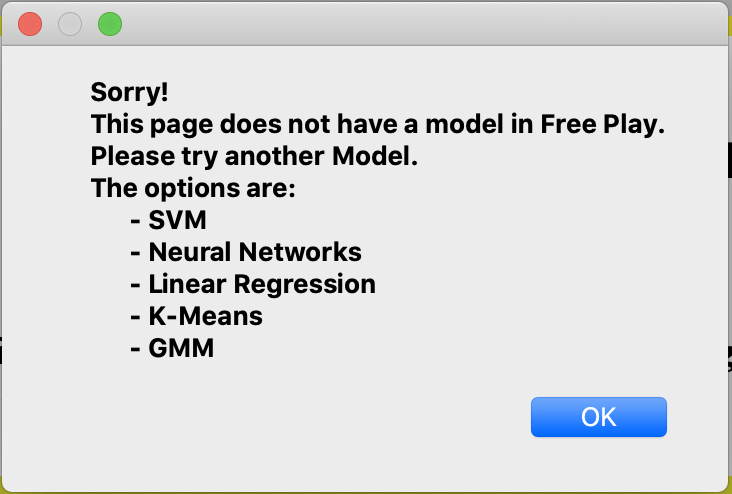
\includegraphics[width=6cm]{graphics/no_model_warning.png}
			\caption{An image displaying the warning message displayed to users.}
			\label{fig:no_model_warning}
		\end{center}
	\end{figure}
	
		When the player clicks the free play button, the application checks the HTML documents title tag and loads up the required model in the free play section. However, if the player clicks the button and the web page does not have a model available, within the free play section or it is just a general overview page, a message box will appear. The message box intension is to let the user know that they can not progress to the free play zone and a list of the available models (see fig: \ref{fig:no_model_warning}).
	
		The Quiz area is an additional area to the learning zone. The Quiz area is where the user can get tested on what they learned in the LZ area, in the form of a multiple-choice quiz. When the user is viewing a topic on the LZ, and they decide to take a quiz, the user will click on the quiz button, and this will read the title tags of the HTML document and open the required quiz. The quiz questions and answers are within their text file, and the name of the file matches the title tag's content. The text file itself holds the information in the format of a 2D array, that has the question at position zero, the answer at position one and then position 2 to 5 are the multiple-choice options. This information from the text file populates a question label and four buttons, allowing the user to click what button they think is the answer. The total of correct answers get added up and displayed to the user at the end in a message box.
	
	\subsection{Free Play Area}
	
		The Free Play (FP) zone is an area where the user gets to interact and play with different ML models. The models include Linear Regression, K-Means, Neural Networks, Linear Discriminant Analysis, Gaussian Mixture Models and SVM. The intension for the FP zone was to have all the models explained in the learning zone be available for the player to interact with, so it could help them fully understand how the model works by allowing the user to manipulate parameters and data points. However, due to time restrictions, there are only six models available, with 5 of the models having real interactivity but to different degrees.
		
		When the FP zone is accessed, unless accessed through the Learning Zone, a randomly selected model gets displayed to the user from the list mentioned before. On first glance, the user has multiple areas to either interact with or present information to them. The screen has a Widget that is linked to a Matplotlib library to handle PyQT5 backend interactions. Also, a model overview is displayed next to the widget, it tells the user information about the model, for example, the type of learning it is, supervised or unsupervised, the name of the model and a brief overview of the model. Just beneath the widget and overview is a group box that contains all the settings for the model and data interaction. The model settings group box contains combo boxes, radio buttons, checkboxes,  line edits and buttons, which all do different things depending on the model and data sets selected. Within the model settings group box, there are three additional group boxes. These are 'Model Attribute(s), 'Model Parameter(s)' and 'Data Options' with each group box displaying different content depending upon the model and data options selected in the combo boxes.
		
		\begin{figure}[t]
			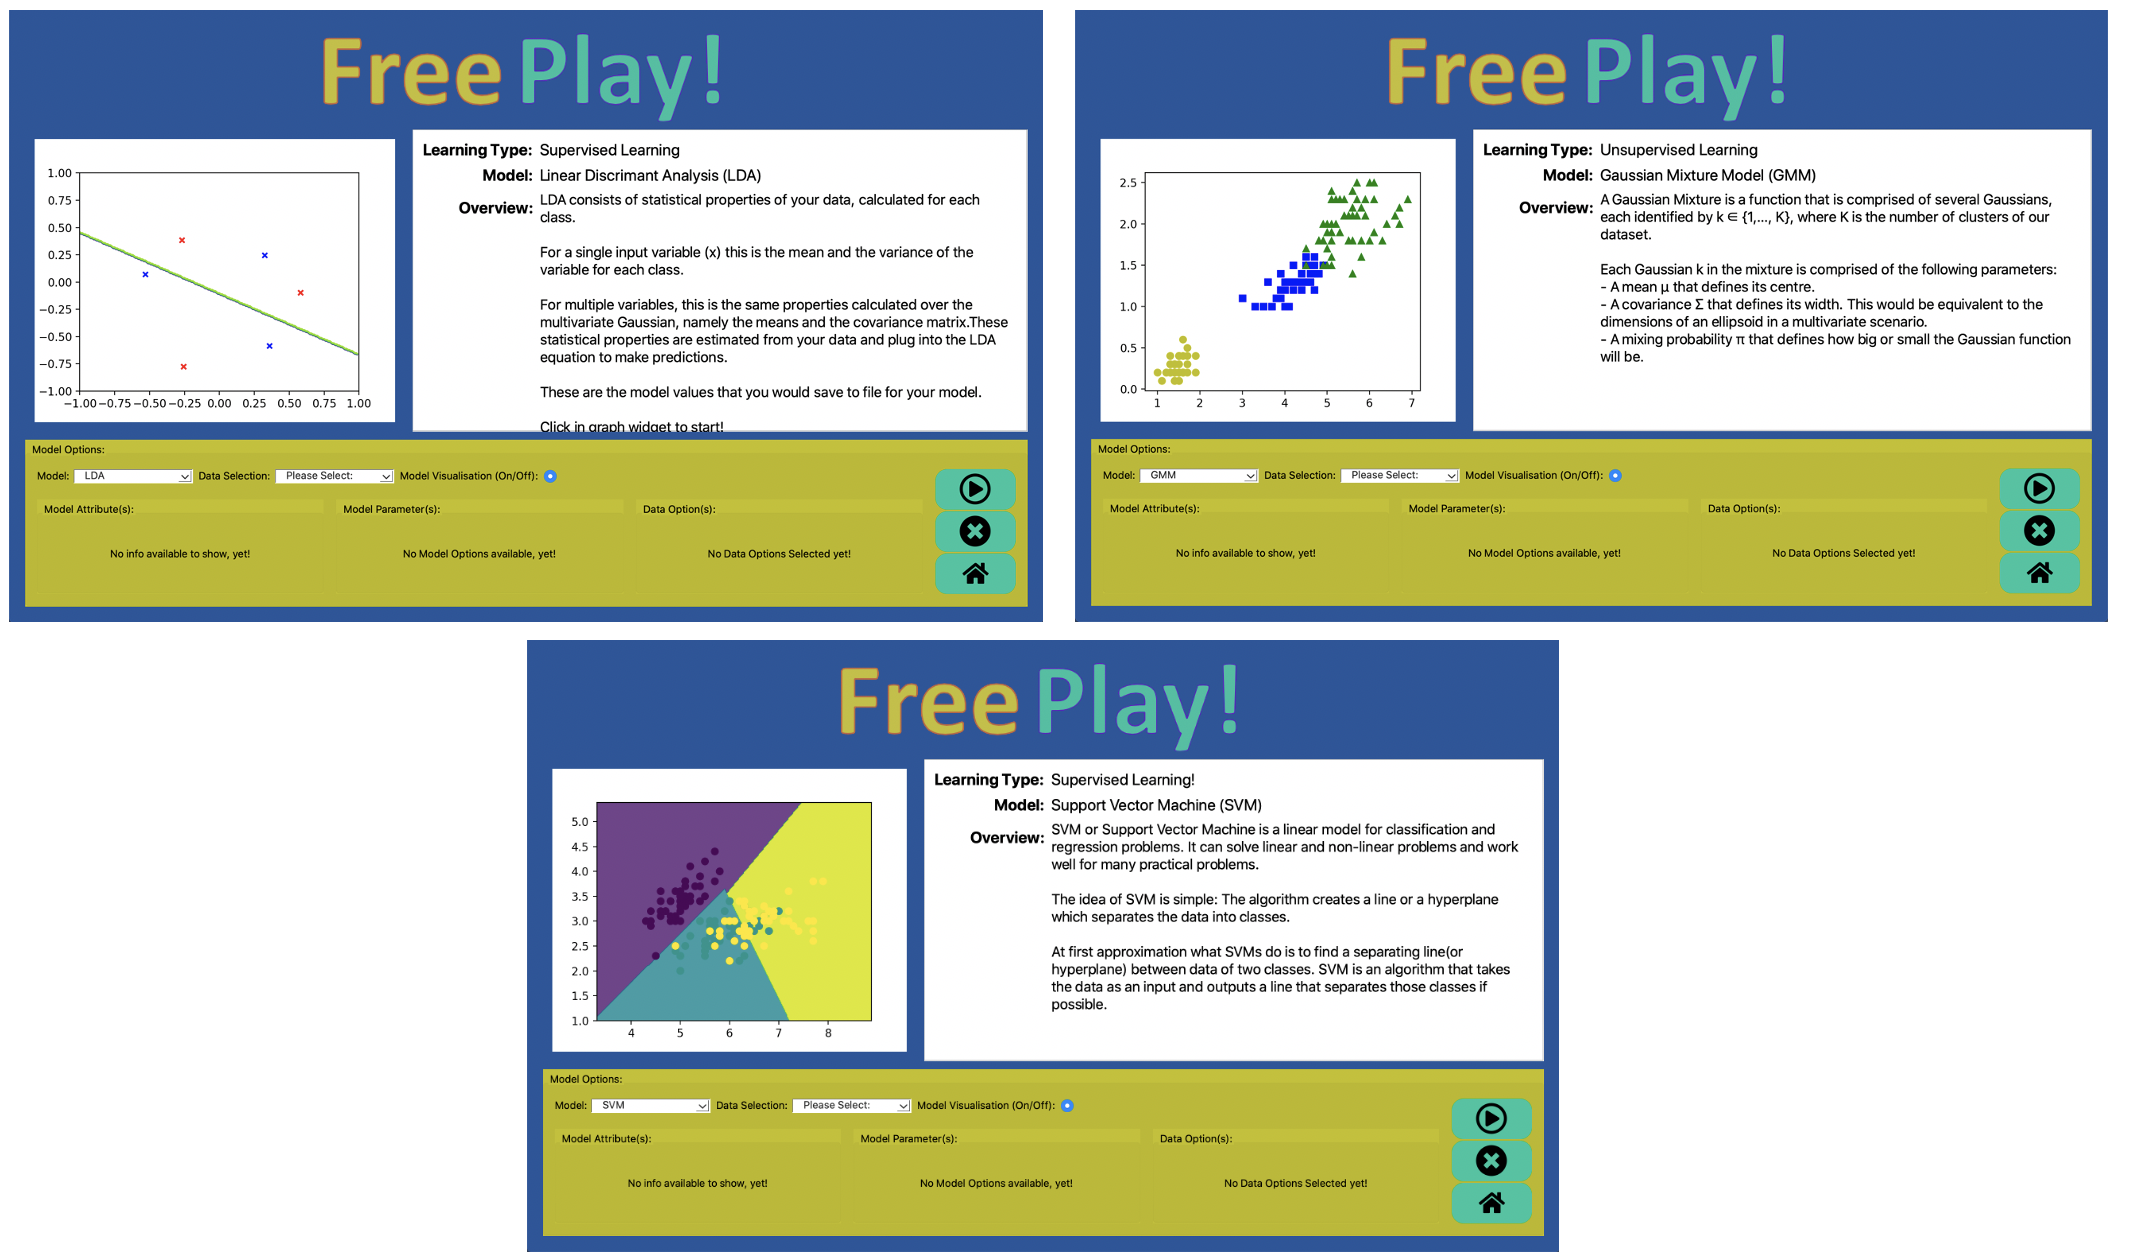
\includegraphics[width=15cm]{graphics/remaining_fp_examples.png}
			\caption{SVM, LDA and GMM UI screens.}
			\label{fig:km_example}
		\end{figure}
		
		The model combo box contains six values, and these are 'Please Select', 'K-Means', 'LDA', 'Linear Regression', 'GMM', 'SVM', 'Neural Networks'. Once one of these options is selected, apart from the 'Please Select', the desired model will display in the Matplotlib widget area. The Model attributes and parameters boxes will display the required information unless the models 'LDA', 'SVM' and 'GMM' are selected (see fig: \ref{}). Instead, a label placeholder saying, 'No Options available, yet!' will be displayed. While LDA has a fully interactive model in the MatplotLib widget, it does not present options for the user to change within the model, the user can only click on the widget and place points, which the model will then apply and create the required actions. Therefore a place holder label appears stating to click in the game widget to interact with the model. While LDA and GMM both have the ability for the model visualisations to toggle on and off, showing how the models have fit their data, GMM has little much additional functionality. GMM only allows the user to toggle on and off the visualisation, which is the model predicting the 'Iris' dataset clusters. However, SVM only displays the model's output, again using the 'Iris' data set, but the output shows the boundary lines and area that each partition covers.
		
		While on the other hand, the Linear Regression, K-Means and Neural Network models display different options. Linear Regression displays to the user labels in the attributes group box to show them the values for the intercept, estimated coefficient and outcome. There is also a line edit available for the user to input a value and see what the model would predict out, which gets displayed in the output label. However, Linear Regression does not have any model parameters, and this is due to the values getting deemed as not having much impact on the model and limited implementational time. 
		
		\begin{figure}[t]
			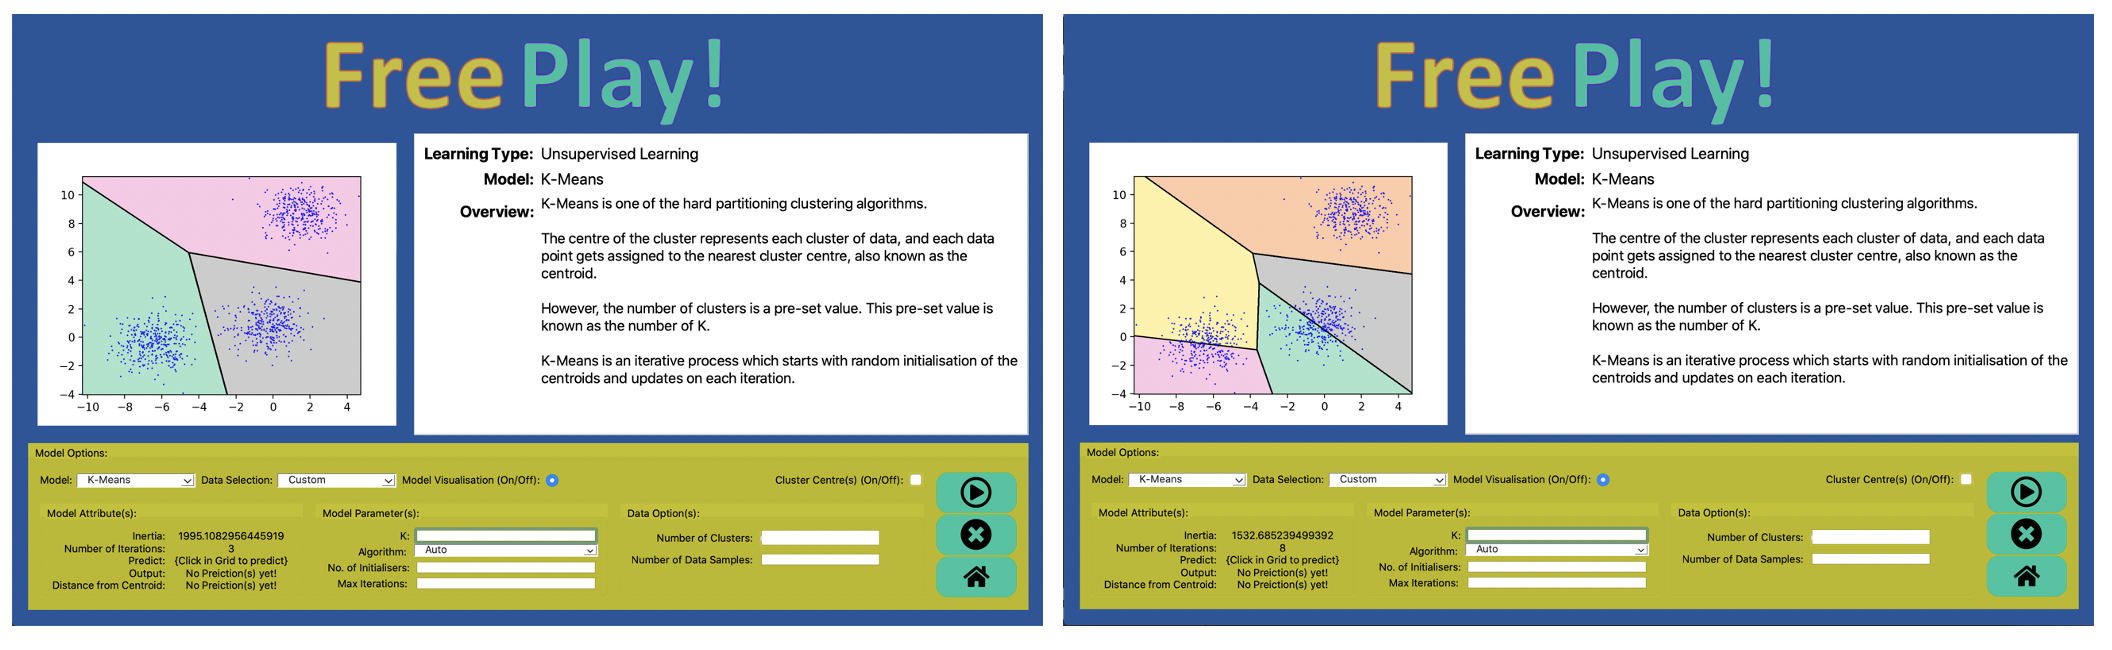
\includegraphics[width=15cm]{graphics/chaning_k_fp_example.png}
			\caption{A comparison of the K-Means k value unchanged ($k=3$) when creating the dataset and then being changed by the user ($k=5$).}
			\label{fig:km_example}
		\end{figure}
		
		When K-Means gets selected (see fig: \ref{fig:km_example}), both the attributes and parameters group boxes have information and selection options displayed to the user. The attributes group box displays the information for Inertia, the number of iterations that got performed fitting the data, prediction, which relies on the user to click within the Matplotlib widget and the X and y coordinates get displayed along with a cluster prediction label in the output label. There is also a distance from the centroid value displayed, and this value got achieved by using the SKLearn Metrics library. The model parameters group box displays multiple line edits and a combo box that allows the user to input values to the model. These will alter the K-Means k value (number of clusters), the number of initialisers, the max number of iterations and the underlying algorithm (auto, full or Elkan), that gets used.  The k value is independent of the number of clusters in the data options, so they do not impact on each other. Allowing the k value to be changed independently will allow the user to be able to experiment with the model to see how two, three or other k values affect the prediction, even when known that the data may have, for example, five different clusters. K-Means also brings up an additional option, and this is to be able to switch on and off the centres of the clusters. When the checkbox gets enabled, this will lay on top of the data points an 'X' where each of the cluster centres is and when it is disabled, it will remove the 'X'.
		
	
		[NN Att no. of layers/ neurons -> params set the values. Not implemented in-app yet!]
		
		The data combo box displays the data options for the different models and depending on what option is selected depends on the information that is on offer to the user in the data options group box. If the custom data option is selected, then the group box will display different options to the user to be able to generate custom data points to be displayed in the Matplotlib widget game screen. The only models that have this option are the Linear Regression and K-Means models. Linear Regression has the data options 'Diabetes' and 'Boston House Prices' and K-Means has the data options 'Iris' and 'Moons'. When these are selected, the data option displays radio button options for the user to select the features they would like the model to display, on the X and y-axis, and get fitted. Linear Regression's 'Custom' data option allows the user the ability to change the random generated data's settings. These settings include the number of data samples and if there are any outliers wanted, if so then an option to add the number of outliers. Whereas K-Means 'Custom' data option allows the user the ability to change the number of clusters to generate and the number of data samples wanted. The other models have a label placeholder saying, 'no data options selected yet!' and no actual data selection options. In the case of LDA and Neural Network, this is more due to the decision we made. Based on the way the model's fit function was implemented, not allowing the user to generate random data was decided. Doing so would impact on how the model gets interacted with by the user. However, in the case of the other models, it was a lack of time that impacted the inability to add this feature. Though, it was always the intention to add it.
		
		The final aspects of the Model options group box are three buttons, a play button, a clear button and a home button. Where the home button is self-explanatory in terms of returning the user to the main menu, and the clear button resetting the Matplotlib Widget axis contents. The play button is where the primary handling of how the user interacts with the back end of the models and datasets. When the user inputs information, they are required to press the play button for these features to be implemented.
	
	
	
	\subsection{Achievements Area}
	The intensions for the Achievement Area was displaying to the user all of the gamification badges available. Providing an overview and hits on how to unlock them. The achievements were going to have a bronze, silver and gold level, and we planned to be unlocked once the user had completed specific tasks like playing the game three times or completing a quiz. However, due to time limitation, this was not possible, and the application, as it currently stands, displays a coming soon image and button for the user to navigate back to the main menu.
	
	
	\section{Example user stories (A UML term for case studies or example playthroughs)}
	\label{sec:ide_used}
	
	
	
